\section{Ciclo gonotrófico}
\label{sec:tasa-ciclo-gonotrofico}
Para el análisis de la tasa de desarrollo, en días, del ciclo gonotrófico de las hembras del Aedes
aegypti, se clasificó la población en hembras núliparas y paridas. En la
\tabref{tab:ciclo-gonotrofico-test} se puede observar una media de $5,03$ días para las hembras
nulíparas y  $2,92$ días para las paridas para una temperatura aproximada de $25,11$ \textcelsius.

\begin{table}[!htbp]
    \begin{minipage}{\textwidth}
        \centering
        \caption{ \label{tab:ciclo-gonotrofico-test} Análisis de duración del ciclo gonotrófico
        de la hembra de Aedes aegypti nueve temperaturas constantes  (18-34 \textcelsius).}
        \begin{tabular}{l *{10}{c} }
            \hline \\
            & &  & &  & &  &  &  &  & Media\\
            Población & 18\textcelsius & 20 \textcelsius & 22 \textcelsius & 24 \textcelsius
                      & 25 \textcelsius & 26\textcelsius  & 27 \textcelsius & 30 \textcelsius
                      & 34\textcelsius & General\\

            \hline
            \hline \\
            Nulíparas\footnote{Hembras nulíparas que no han ovipuesto.}
                        & 8,97 & 7,4  & 6,13  & 5,08  & 4,63 & 4,22  & 3,85 & 2,94 & 2,06 & 5,03\\
            Paridas\footnote{Hembras que ya han realizado al menos una ovipostura.}
                        & 5,21 & 4,3  & 3,56  & 2,95  & 2,69 & 2,45  & 2,24 & 1,71 & 1,2 & 2,92\\
            Media \footnote{Promedio general de la duración general del ciclo gonotrófico para las
            hembras}
                        & 7,09 & 5,85 & 4,85  & 4,02  & 3,66 & 3,34  & 3,05 & 2,33 & 1,63 & 3,98\\
        \end{tabular}
    \end{minipage}
\end{table}

Las variaciones en la temperatura influyen en tiempo de digestión de la sangre y el
desarrollo de los ovarios, a medida que la temperatura desciende, la digestión y por ende el ciclo
gonotrófico tomará más tiempo (\figref{fig:ciclo-gonotrofico-temperatura}). En \cite{edman1987host}
se observó que hembras nulíparas de Aedes aegypti poseen un proceso de digestión es más lento en
las hembras paridas y por ende el ciclo gonotrófico de las mismas tiene a ser más largo. Existen
diversos estudios, que han reportado que el patrón diario de alimentación de los mosquitos, varia
de acuerdo a las localidades y subespecies. A continuación se mencionaran algunos estudios
realizados correspondientes a la duración del ciclo gonotrófico, con el fin de realizar una
comparación con los resultados obtenidos mediante el proceso evolutivo.

\begin{figure}[!htbp]
    \centering
    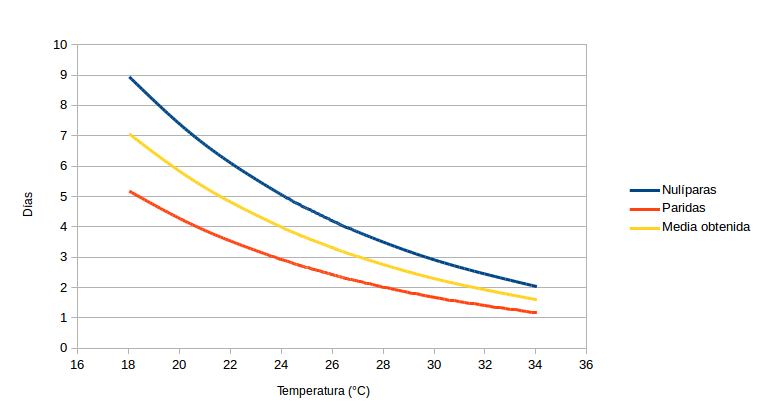
\includegraphics[width=1\textwidth]{capitulo-6/graphics/ciclo-gonotrofico-temperatura.png}
    \caption{\label{fig:ciclo-gonotrofico-temperatura} Tasa de desarrollo, en días, del ciclo
    gonotrófico de hembras nulíparas, hembras paridas y la media general a nueve temperaturas
    constantes (18-34 \textcelsius).}
\end{figure}

En \cite{beltran2001bionomia} se determinó que la duración del ciclo gonotrófico del Aedes
aegypti, para los siguientes municipios de México en, 3 días para Tamazula de Gordiano a una
temperatura de $21,5$ \textcelsius, 3 días para Techaluta de Montenegro a $22,8$ \textcelsius, 4
días para Tuxpan a 22 \textcelsius y 5 días para CD Zacoalco de Torres a $22,7$ \textcelsius.

En \cite{luevano1993ciclo}, el autor determinó la duración del ciclo gonotrófico de las
poblaciones naturales de Aedes aegypti en el área metropolitana de Monterrey, Nuevo León. México,
en cinco días, a una temperatura promedio de $25,5$ \textcelsius.

En \cite{trpis1986dispersal} los autores reportaron una duración del ciclo gonotrófico en Kenia a
nivel rural de, 5 a 7 días para el primer ciclo (hembras nulíparas) y de 4 a 5 días para los
siguientes ciclos (hembras paridas). El método utilizado fue de captura con cebo humano de
mosquitos de Aedes aegypti.

Según \cite{sivanathan2006ecology} el ciclo gonotrófico del aAedes aegypti y Aedes albopictus se
encuentra acotada entre $2,73$ a 3 días respectivamente.

Las diferentes condiciones climáticas y la capacidad de adaptación en habitad específicos, del
Aedes aegypti, son las responsables de diferencias que se puedan tener entre cepas del mosquito.
La duración del ciclo gonotrófico obtenida, depende de los coeficientes para el modelo de
maduración enzimática de \cite{sharpe1977reaction} que fue tomado de \cite{otero2006stochastic},
que según los autores fue tomado de \cite{focks1993dynamic}.

